\section{Homework 5}

\begin{exercise}
    [P46, Ex2] Prove that \(\Phi^\vee\) is a root system in \(E\), whose Weyl group is naturally isomorphic to \(W\). Show also that
    \[
        \langle \alpha^\vee,\beta^\vee\rangle=\langle \beta,\alpha\rangle,
    \]
    and draw a picture of \(\Phi^\vee\) in the cases \(A_1\), \(A_2\), \(B_2\), and \(G_2\).
\end{exercise}

\begin{proof}
    Let \(\Phi\) be a root system in the Euclidean space \(E\). For
    \(\alpha\in \Phi\), put
    \[
        \alpha^\vee=\frac{2\alpha}{(\alpha,\alpha)}.
    \]
    We shall prove that
    \[
        \Phi^\vee:=\{\alpha^\vee\mid \alpha\in\Phi\}
    \]
    is again a root system in \(E\).
    
    First observe that
    \[
        (\alpha^\vee,\alpha^\vee)
        =
        \left(\frac{2\alpha}{(\alpha,\alpha)},
              \frac{2\alpha}{(\alpha,\alpha)}\right)
        =
        \frac{4}{(\alpha,\alpha)}.
    \]
    Hence
    \[
        (\alpha^\vee)^\vee
        =
        \frac{2\alpha^\vee}{(\alpha^\vee,\alpha^\vee)}
        =
        \frac{2\cdot 2\alpha/(\alpha,\alpha)}
             {4/(\alpha,\alpha)}
        =
        \alpha.
    \]
    Thus the map \(\alpha\mapsto \alpha^\vee\) is a bijection from
    \(\Phi\) onto \(\Phi^\vee\). It follows that \(\Phi^\vee\) is finite,
    does not contain \(0\), and spans \(E\), since \(\Phi\) spans \(E\).
    
    Next, suppose \(c\alpha^\vee\in \Phi^\vee\), with \(c\in\mathbb R\).
    Then \(c\alpha^\vee=\beta^\vee\) for some \(\beta\in\Phi\). Hence
    \(\beta^\vee\) is proportional to \(\alpha^\vee\), and therefore \(\beta\)
    is proportional to \(\alpha\). Since \(\Phi\) is reduced,
    \[
        \beta=\pm\alpha.
    \]
    Therefore
    \[
        \beta^\vee=\pm\alpha^\vee,
    \]
    so \(c=\pm 1\). Thus the only multiples of \(\alpha^\vee\) in
    \(\Phi^\vee\) are \(\pm\alpha^\vee\).
    
    We now check stability under reflections. Since \(\alpha^\vee\) is a positive
    scalar multiple of \(\alpha\), the reflecting hyperplanes are the same:
    \[
        P_{\alpha^\vee}=P_\alpha.
    \]
    Thus
    \[
        s_{\alpha^\vee}=s_\alpha.
    \]
    For \(\beta\in\Phi\), since \(s_\alpha\) is orthogonal, we get
    \[
        s_{\alpha^\vee}(\beta^\vee)
        =
        s_\alpha\left(\frac{2\beta}{(\beta,\beta)}\right)
        =
        \frac{2s_\alpha(\beta)}{(s_\alpha\beta,s_\alpha\beta)}
        =
        (s_\alpha\beta)^\vee.
    \]
    But \(s_\alpha(\beta)\in\Phi\), so
    \[
        s_{\alpha^\vee}(\beta^\vee)\in\Phi^\vee.
    \]
    Hence \(\Phi^\vee\) is stable under all reflections \(s_{\alpha^\vee}\).
    
    Finally, for \(\alpha,\beta\in\Phi\),
    \[
    \begin{aligned}
        \langle \alpha^\vee,\beta^\vee\rangle
        &=
        \frac{2(\alpha^\vee,\beta^\vee)}
             {(\beta^\vee,\beta^\vee)}                                      \\[4pt]
        &=
        \frac{
            2\left(
            \frac{2\alpha}{(\alpha,\alpha)},
            \frac{2\beta}{(\beta,\beta)}
            \right)}
            {4/(\beta,\beta)}                                                \\[4pt]
        &=
        \frac{2(\alpha,\beta)}{(\alpha,\alpha)}                              \\[4pt]
        &=
        \langle \beta,\alpha\rangle.
    \end{aligned}
    \]
    Since \(\langle \beta,\alpha\rangle\in\mathbb Z\), we have
    \[
        \langle \alpha^\vee,\beta^\vee\rangle\in\mathbb Z.
    \]
    Therefore \(\Phi^\vee\) satisfies all root system axioms.
    
    The Weyl group \(W^\vee\) of \(\Phi^\vee\) is generated by the reflections
    \(s_{\alpha^\vee}\). But \(s_{\alpha^\vee}=s_\alpha\), so
    \[
        W^\vee=\langle s_{\alpha^\vee}\mid \alpha\in\Phi\rangle
        =
        \langle s_\alpha\mid \alpha\in\Phi\rangle
        =
        W.
    \]
    Thus the Weyl group of \(\Phi^\vee\) is naturally isomorphic to \(W\);
    in this realization it is literally the same subgroup of \(GL(E)\).
    
    For the pictures below, long coroots are drawn thicker. The diagrams use
    the fact that dualizing preserves \(A_1,A_2\), interchanges \(B_2\) and
    \(C_2\), and sends \(G_2\) to an isomorphic \(G_2\) with long and short
    roots interchanged.
    
    \begin{center}
    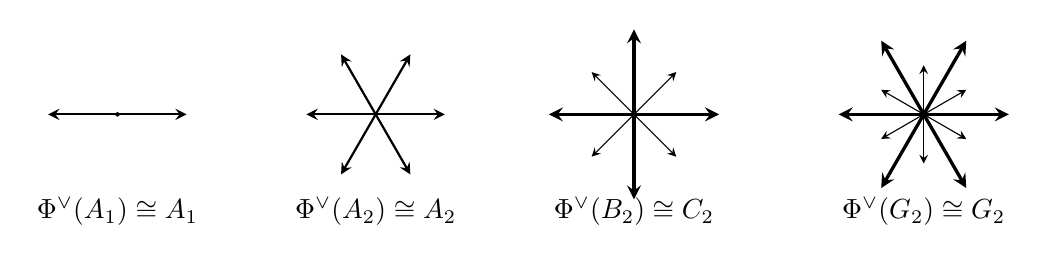
\begin{tikzpicture}[scale=0.8, root/.style={->,>=stealth}]
        % A1
        \begin{scope}[shift={(0,0)}]
            \foreach \a in {0,180}{
                \draw[root,thick] (0,0) -- ({1.1*cos(\a)},{1.1*sin(\a)});
            }
            \fill (0,0) circle (1pt);
            \node at (0,-1.55) {\(\Phi^\vee(A_1)\cong A_1\)};
        \end{scope}
    
        % A2
        \begin{scope}[shift={(4.1,0)}]
            \foreach \a in {0,60,...,300}{
                \draw[root,thick] (0,0) -- ({1.1*cos(\a)},{1.1*sin(\a)});
            }
            \fill (0,0) circle (1pt);
            \node at (0,-1.55) {\(\Phi^\vee(A_2)\cong A_2\)};
        \end{scope}
    
        % B2 dual = C2
        \begin{scope}[shift={(8.2,0)}]
            \foreach \a in {0,90,180,270}{
                \draw[root,very thick] (0,0) -- ({1.35*cos(\a)},{1.35*sin(\a)});
            }
            \foreach \a in {45,135,225,315}{
                \draw[root,thin] (0,0) -- ({0.95*cos(\a)},{0.95*sin(\a)});
            }
            \fill (0,0) circle (1pt);
            \node at (0,-1.55) {\(\Phi^\vee(B_2)\cong C_2\)};
        \end{scope}
    
        % G2 dual
        \begin{scope}[shift={(12.8,0)}]
            \foreach \a in {0,60,...,300}{
                \draw[root,very thick] (0,0) -- ({1.35*cos(\a)},{1.35*sin(\a)});
            }
            \foreach \a in {30,90,...,330}{
                \draw[root,thin] (0,0) -- ({0.78*cos(\a)},{0.78*sin(\a)});
            }
            \fill (0,0) circle (1pt);
            \node at (0,-1.55) {\(\Phi^\vee(G_2)\cong G_2\)};
        \end{scope}
    \end{tikzpicture}
    \end{center}
    \end{proof}

\begin{exercise}
    [P54, Ex1] Let \(\Phi^\vee\) be the dual system of \(\Phi\), and let
    \[
        \Delta^\vee=\{\alpha^\vee\mid \alpha\in\Delta\}.
    \]
    Prove that \(\Delta^\vee\) is a base of \(\Phi^\vee\). [Compare Weyl chambers of \(\Phi\) and \(\Phi^\vee\).]
\end{exercise}

\begin{proof}
    Let
    \[
        \Delta=\{\alpha_1,\ldots,\alpha_\ell\}
    \]
    be a base of \(\Phi\), and put
    \[
        \Delta^\vee=\{\alpha_1^\vee,\ldots,\alpha_\ell^\vee\}.
    \]
    We prove that \(\Delta^\vee\) is a base of \(\Phi^\vee\).
    
    First, since
    \[
        \alpha_i^\vee=\frac{2\alpha_i}{(\alpha_i,\alpha_i)}
    \]
    is a positive scalar multiple of \(\alpha_i\), the set \(\Delta^\vee\) is a basis
    of \(E\), because \(\Delta\) is a basis of \(E\).
    
    Now compare the Weyl chambers of \(\Phi\) and \(\Phi^\vee\). For a root
    \(\alpha\), let
    \[
        P_\alpha=\{\lambda\in E\mid (\lambda,\alpha)=0\}
    \]
    be the reflecting hyperplane. Since \(\alpha^\vee\) is a positive scalar multiple
    of \(\alpha\), we have
    \[
        P_{\alpha^\vee}=P_\alpha.
    \]
    Therefore the hyperplane arrangements
    \[
        \bigcup_{\alpha\in\Phi}P_\alpha
        \qquad\text{and}\qquad
        \bigcup_{\alpha^\vee\in\Phi^\vee}P_{\alpha^\vee}
    \]
    are identical. Hence \(\Phi\) and \(\Phi^\vee\) have the same Weyl chambers.
    
    Let \(C\) be the fundamental Weyl chamber corresponding to \(\Delta\):
    \[
        C=\{\lambda\in E\mid (\lambda,\alpha_i)>0,\;1\leq i\leq \ell\}.
    \]
    Because \(\alpha_i^\vee\) is a positive scalar multiple of \(\alpha_i\), this is
    also
    \[
        C=\{\lambda\in E\mid (\lambda,\alpha_i^\vee)>0,\;1\leq i\leq \ell\}.
    \]
    Thus the same chamber \(C\) is bounded by the walls
    \[
        P_{\alpha_1}=P_{\alpha_1^\vee},\ldots,
        P_{\alpha_\ell}=P_{\alpha_\ell^\vee}.
    \]
    
    By the standard correspondence between Weyl chambers and bases, the base
    attached to a chamber consists of the unique positive roots perpendicular to
    the walls of that chamber. For the chamber \(C\) in the root system \(\Phi\),
    these roots are
    \[
        \alpha_1,\ldots,\alpha_\ell.
    \]
    For the same chamber \(C\) in the dual root system \(\Phi^\vee\), the unique
    positive root perpendicular to \(P_{\alpha_i}=P_{\alpha_i^\vee}\) is
    \[
        \alpha_i^\vee.
    \]
    Indeed, if \(\beta^\vee\in\Phi^\vee\) is perpendicular to the same wall as
    \(\alpha_i^\vee\), then \(\beta^\vee\) is a scalar multiple of \(\alpha_i^\vee\),
    so by the root system axiom it is \(\pm\alpha_i^\vee\). The positivity condition
    with respect to \(C\) selects \(\alpha_i^\vee\), not \(-\alpha_i^\vee\).
    
    Hence the base of \(\Phi^\vee\) associated with the chamber \(C\) is precisely
    \[
        \Delta^\vee=\{\alpha^\vee\mid \alpha\in\Delta\}.
    \]
    Therefore \(\Delta^\vee\) is a base of \(\Phi^\vee\).
    \end{proof}

\begin{exercise}
    [P54, Ex10] Given \(\Delta=\{\alpha_1,\ldots,\alpha_\ell\}\) in \(\Phi\), let
    \[
        \lambda=\sum_{i=1}^{\ell} k_i\alpha_i,
    \]
    where \(k_i\in\mathbb{Z}\) and either all \(k_i\geq 0\) or all \(k_i\leq 0\). Prove that either \(\lambda\) is a multiple (possibly \(0\)) of a root, or else there exists \(\sigma\in W\) such that
    \[
        \sigma\lambda=\sum_{i=1}^{\ell} k_i'\alpha_i,
    \]
    with some \(k_i'>0\) and some \(k_i'<0\).

    \emph{Sketch of proof.} If \(\lambda\) is not a multiple of any root, then the hyperplane \(P_\lambda\) orthogonal to \(\lambda\) is not included in \(\bigcup_{\alpha\in\Phi}P_\alpha\). Take
    \[
        \mu\in P_\lambda-\bigcup_{\alpha\in\Phi}P_\alpha.
    \]
    Then find \(\sigma\in W\) for which all \((\alpha_i,\sigma\mu)>0\). It follows that
    \[
        0=(\lambda,\mu)=(\sigma\lambda,\sigma\mu)
        =\sum k_i'(\alpha_i,\sigma\mu).
    \]
\end{exercise}

\begin{proof}
    Let
    \[
        \Delta=\{\alpha_1,\ldots,\alpha_\ell\}
    \]
    be a base of \(\Phi\), and let
    \[
        \lambda=\sum_{i=1}^{\ell}k_i\alpha_i,
    \]
    where the \(k_i\in\mathbb Z\) are either all nonnegative or all nonpositive.
    
    If \(\lambda=0\), then \(\lambda\) is the zero multiple of any root, so there is
    nothing to prove. Also, replacing \(\lambda\) by \(-\lambda\) does not change
    the assertion: being a scalar multiple of a root is unchanged up to sign, and
    if some Weyl group translate of \(-\lambda\) has coefficients of both signs,
    then the corresponding translate of \(\lambda\) also has coefficients of both
    signs. Hence we may assume that
    \[
        k_i\geq 0
        \qquad
        \text{for all }i.
    \]
    
    Assume now that \(\lambda\) is not a scalar multiple of any root. For
    \(\nu\in E\), write
    \[
        P_\nu=\{\mu\in E\mid (\mu,\nu)=0\}.
    \]
    We claim that
    \[
        P_\lambda\not\subseteq \bigcup_{\alpha\in\Phi}P_\alpha.
    \]
    Indeed, if
    \[
        P_\lambda\subseteq \bigcup_{\alpha\in\Phi}P_\alpha,
    \]
    then, since \(P_\lambda\) is a real vector space and \(\Phi\) is finite, the vector
    space \(P_\lambda\) would be a finite union of the proper subspaces
    \[
        P_\lambda\cap P_\alpha.
    \]
    Over the infinite field \(\mathbb R\), this is impossible unless one of these
    subspaces is all of \(P_\lambda\). Thus for some \(\alpha\in\Phi\),
    \[
        P_\lambda\subseteq P_\alpha.
    \]
    Both are hyperplanes, so
    \[
        P_\lambda=P_\alpha.
    \]
    Consequently \(\lambda\) is a scalar multiple of \(\alpha\), contradicting the
    assumption.
    
    Therefore we can choose
    \[
        \mu\in P_\lambda-\bigcup_{\alpha\in\Phi}P_\alpha.
    \]
    The vector \(\mu\) is regular, since it lies on no root hyperplane. Hence \(\mu\)
    belongs to some Weyl chamber. Since the Weyl group acts simply transitively
    on the Weyl chambers, there exists \(\sigma\in W\) such that \(\sigma\mu\)
    lies in the fundamental chamber corresponding to \(\Delta\). Thus
    \[
        (\alpha_i,\sigma\mu)>0
        \qquad
        \text{for }1\leq i\leq \ell.
    \]
    
    Write
    \[
        \sigma\lambda=\sum_{i=1}^{\ell}k_i'\alpha_i.
    \]
    Because \(W\) preserves the root lattice \(\mathbb Z\Phi=\mathbb Z\Delta\),
    we have
    \[
        k_i'\in\mathbb Z.
    \]
    Since \(\mu\in P_\lambda\), we have
    \[
        (\lambda,\mu)=0.
    \]
    The Weyl group preserves the inner product, so
    \[
    \begin{aligned}
        0
        &=
        (\lambda,\mu)                                                   \\
        &=
        (\sigma\lambda,\sigma\mu)                                       \\
        &=
        \left(\sum_{i=1}^{\ell}k_i'\alpha_i,\sigma\mu\right)             \\
        &=
        \sum_{i=1}^{\ell}k_i'(\alpha_i,\sigma\mu).
    \end{aligned}
    \]
    But every number
    \[
        (\alpha_i,\sigma\mu)
    \]
    is strictly positive. Also \(\sigma\lambda\neq 0\), so not all \(k_i'\) are zero.
    Therefore the integers \(k_i'\) cannot all be nonnegative and cannot all be
    nonpositive. Hence some \(k_i'\) is positive and some \(k_j'\) is negative.
    
    Thus, unless \(\lambda\) is a scalar multiple of a root, there exists
    \(\sigma\in W\) such that
    \[
        \sigma\lambda=\sum_{i=1}^{\ell}k_i'\alpha_i
    \]
    has coefficients of both signs.
    \end{proof}

\begin{exercise}
    Prove that if \(\alpha,\beta\) are roots, \(\beta\neq\pm\alpha\), \(k\) is a real number, and \(\beta+k\alpha\) is a root, then \(k\) is an integer.
\end{exercise}

\begin{proof}
    Let
    \[
        Q=\mathbb Z\Phi
    \]
    be the root lattice. Suppose that
    \[
        \gamma:=\beta+k\alpha
    \]
    is a root. Since \(\beta,\gamma\in\Phi\), we have
    \[
        k\alpha=\gamma-\beta\in Q.
    \]
    
    We recall the standard fact that every root is simple for some choice of base.
    Indeed, fix a base \(\Delta\). If a positive root is not simple, then by the usual
    height-reduction lemma there is a simple root \(\delta\in\Delta\) such that
    \(s_\delta\) lowers its height. Repeating this process sends the root to a
    simple root. Applying the inverse Weyl group element gives a base containing
    the original root. If the original root is negative, apply the same argument
    to its negative and then replace the resulting base by its negative.
    
    Hence there exists a base
    \[
        \Delta'=\{\alpha,\alpha_2,\ldots,\alpha_\ell\}
    \]
    of \(\Phi\) containing \(\alpha\). Since every base is a \(\mathbb Z\)-basis of the
    root lattice, we have
    \[
        Q=\mathbb Z\Delta'
        =
        \mathbb Z\alpha\oplus \mathbb Z\alpha_2\oplus\cdots\oplus
        \mathbb Z\alpha_\ell.
    \]
    Because \(k\alpha\in Q\), there exist integers
    \[
        n_1,n_2,\ldots,n_\ell\in\mathbb Z
    \]
    such that
    \[
        k\alpha
        =
        n_1\alpha+n_2\alpha_2+\cdots+n_\ell\alpha_\ell.
    \]
    Since \(\Delta'\) is a real basis of \(E\), this expression is unique. Comparing
    coefficients in the basis \(\Delta'\), we get
    \[
        k=n_1
        \qquad\text{and}\qquad
        n_2=\cdots=n_\ell=0.
    \]
    Therefore
    \[
        k\in\mathbb Z.
    \]
    
    Thus, if \(\alpha,\beta\in\Phi\), \(\beta\neq\pm\alpha\), and
    \(\beta+k\alpha\in\Phi\) for some \(k\in\mathbb R\), then \(k\) is an integer.
    \end{proof}